\documentclass[twocolumn,twoside,letterpaper]{article} 

\usepackage{color}

\usepackage{geneticsT2}
\usepackage{times}

\addtolength{\oddsidemargin}{-.2cm}
\addtolength{\evensidemargin}{-1.2cm}

\addtolength{\textwidth}{1.5cm}
\addtolength{\topmargin}{-2cm}
\addtolength{\textheight}{3.5cm}

\renewcommand{\textfraction}{0.01}
\renewcommand{\topfraction}{0.99}
\renewcommand{\bottomfraction}{0.65}
\renewcommand{\floatpagefraction}{0.90}
\renewcommand{\dbltopfraction}{0.95}
\renewcommand{\dblfloatpagefraction}{0.80}
\renewcommand{\sfdefault}{phv}

% plr added
\newcommand{\mutrate}{\lambda_{\text{mut}}}
\newcommand{\migrate}{\lambda_{\text{mig}}}
\newcommand{\Tmut}{T_{\text{mut}}}
\newcommand{\Tmig}{T_{\text{mig}}}

\usepackage{fancyhdr}
\pagestyle{fancy}
\fancyhf{}
%\fancyhead[LE,RO]{\thepage}
%\fancyhead[CE]{S. Takuno \emph{et al}.}
%\fancyhead[CO]{Pseudogene preservation by gene conversion}
\fancyfoot[LE,RO]{{\sfbf \thepage}}
\renewcommand{\headrulewidth}{0pt}
\fancypagestyle{plain}{
	\fancyhf{}
}

%editing commands (please leave in for now)
\newcommand{\jri}[1]{\textcolor{blue}{ \emph{\scriptsize  #1}} }
\newcommand{\st}[1]{\textcolor{red}{#1}}
\newcommand{\comst}[1]{\textcolor{red}{ \em{\scriptsize  #1}} }

%\newcommand{\mbh}[1]{\textcolor{green}{\bf #1}}
%\newcommand{\mbh}[1]{\textcolor{green}{ \em{\scriptsize  #1}} }
\definecolor{mattgreen} {rgb} {0,0.6,0}
\newcommand{\mbh}[1]{\textcolor{mattgreen}{ \em{\scriptsize  #1}} }
\definecolor{peterpurple}{rgb}{.6,0,.6}
\newcommand{\plr}[1]{\textcolor{peterpurple}{ \emph{\scriptsize (#1)}} }

\usepackage[normalem]{ulem}
\def\dt{\bgroup
 \markoverwith{\lower-0.2ex\hbox
 {\kern-.03em\vbox{\hrule width.2em\kern0.45ex\hrule}\kern-.03em}}%
 \ULon}
\MakeRobust\dt
\usepackage[normalem]{ulem}
\def\dt{\bgroup
 \markoverwith{\lower-0.2ex\hbox
 {\kern-.03em\vbox{\hrule width.2em\kern0.45ex\hrule}\kern-.03em}}%
 \ULon}
\MakeRobust\dt

%%%%

%\title{The molecular basis of parallel adaptation to highland climate\\ in maize domesticated populations}
\title{The molecular basis of parallel adaptation to\\ highland climate in domesticated maize}
\author{
 \small\sfbf{Shohei Takuno$^{\ast}$, Peter Ralph$^{\dag, \ddag}$, Sofiane Mezmouk$^{\ast}$, Kelly Swarts$^{\S}$, Rob J. Elshire$^{\S}$, Jeffrey C. Glaubitz$^{\S}$,}\\
   \small\sfbf{Edward S. Buckler$^{\S, \ast\ast}$, Matthew B. Hufford$^{\ast}$, and Jeffrey Ross-Ibarra$^{\ast,\dag\dag,}$}\thanks{
Corresponding author:  Department of Plant Sciences, University of California, Davis, California 95616, USA. 
    E-mail: \mbox{rossibarra@ucdavis.edu}}\\[0.3cm]
   % \jri{note change to author order}
   \small\sf $^{\ast}$Department of Plant Sciences, University of California, Davis, California 95616, USA,\\
   \small\sf $^\dag$ Department of Evolution and Ecology, University of California, Davis, California 95616, USA,\\
   \small\sf $^\ddag$Department of Biological Sciences, University of Southern California,  Los Angeles,California 90089-0371, USA,\\
   \small\sf $^\S$Institute for Genomic Diversity, Cornell University, Ithaca, New York 14853-2703, USA,\\
   \small\sf $^{\ast\ast}$US Department of Agriculture�Agriculture Research Service (USDA-ARS) \st{address},\\
   \small\sf $^{\dag\dag}$The Center for Population Biology and the Genome Center, University of California, Davis, California 95616 , USA\\
}
%\begin{flushright}
%\end{flushright}
   
\date{Revised manuscript for \emph{Genetics}, \today}

\abstract{
Parallel adaptation is defined as independent colonization of multiple species/subpopulations to similar environments via adaptive mutations in the same gene.
To understand the molecular basis of parallel adaptation, the adaptive process to highland climates of domesticated maize (\emph{Zea mays} ssp. \emph{mays}) in Mexico and South America was investigated.
After its domestication in the Balsas River Valley in the Mexico lowlands, maize spread quickly across the Americas.  
Adaptation to highland climates in Mexico and South America occurred independently from locally-adapted lowland maize.  
Here, we show the result of a genome scan to identify loci involved in parallel adaptation to highland climates.  
To do this, we generated two large SNP data sets of 94 maize landraces, sampled from Mexico and South America.  
We first inferred the demographic history of these lowland and highland populations.  
We used the inferred demographic history to then perform a genome scan to identify highly differentiated loci that may have contributed to adaptation to highland climates.  
The majority of loci identified showed evidence of selection in highland habitats from standing variation, yet we saw little evidence of parallel adaptation.  
%insert the result of GWAS by Sofiane, here
We discuss the significance of these results in the context of the molecular basis of adaptation to new environments. }

\usepackage{natbib}
\bibpunct{(}{)}{;}{a}{}{,}

\usepackage{amsmath}

\usepackage{graphicx}

\begin{document}

\maketitle

%Once concern repeatedly raise by G. Coop is how many selected loci we may be missing. Is this a reasonable back-of-the-envelop?:
%
%width<-function(s,c){ return(0.01*s/c) } ##uses width of diversity reduction in sweep result. better result to use?
%
%prob<-function(s,c){ return(width(s,c)*snps*2/2.3E9) }
%twice width to include either side of SNP
%
%loci=1:100
%pbinom(round(loci/2,0),loci,prob(0.01,1E-8))
%
%that gives us that we should pick up majority of strongly selected sites (s=0.01) but for weaker selection (s=0.001) our chance of missing all the sites remains substantial until number of selected sites >>50




%   INTRODUCTION   %
\noindent Parallel adaptation is defined as a process in which multiple species or subpopulations adapt to similar environments independently. %can we really say "independently" under the second scenario of standing variation? is it independent if they use the same standing variant? do we need to call it something else?
Parallel adaptation occurs via independent beneficial mutations at the same locus, whereas adaptation via beneficial mutations producing the same phenotypic effect through different genes can be referred to as convergent evolution \cite[]{Wood_2005_15881688,Arendt_2008_18022278,Elmer_2011_21459472}.  
Recent molecular studies have provided evidence for parallel adaptation in a wide range of species, \emph{e.g.}, malaria resistance \cite[]{Currat_2002_11741197,Kwiatkowski_2005_16001361} and lactase persistence \cite[]{Tishkoff_2007_17159977} in humans, adaptation to freshwater environments in three-spined sticklebacks \cite[]{Colosimo_2005_15790847}, and insecticide resistance in several species  \cite[]{Ffrench_2000}.

At the molecular level, parallel adaptation can be achieved in at least three ways.  
To explain these, we introduce a simple population divergence model (Figure~\ref{fig1}).  
We consider that two derived populations are differentiated from a parental population and adapt to similar environments.  
In our first example, a beneficial mutation independently arises and reaches fixation by natural selection in the two derived populations (Pattern A in Figure~\ref{fig1}).  
Malarial resistance in humans is an example of this first scenario, as mutations from Glu to Val at the sixth codon of the $\beta$-globin gene have occurred on multiple unique haplotypes  \cite[]{Currat_2002_11741197,Kwiatkowski_2005_16001361}.  
Secondly, parallel adaptation can occur from standing variation (Pattern B). %see comment above about whether this is "independent"
In threespine sticklebacks, for example, selection has repeatedly acted to reduce armor plating during colonizations of freshwater environments.  In most cases, adaptation in these populations took advantage of standing variation for the low-plated morph in marine populations \cite[]{Colosimo_2005_15790847}.  
Lastly, in Pattern C, different adaptive mutations arise within the same gene in each population to produce the same phenotypic effect.  
Similar grain fragrance phenotypes in rice across several parts of East Asia, for example, are due to at least eight distinct loss-of-function alleles in the gene \emph{BADH2}\cite[]{Kovach_2009_19706531}:  

%%%%%%%%%%%%%%%%%%%%%%%%%%%%%%%%%%%%%%%%%% FIGURE
\begin{figure}[tb]   
  \begin{center}
   \vspace{-0mm}
   %\includegraphics[width=0.23\textwidth]{figs/model}
   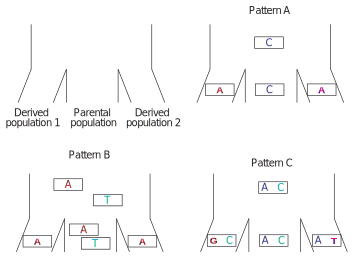
\includegraphics[width=0.4\textwidth]{fig/Fig1-4}
   \renewcommand{\baselinestretch}{0.9}
   \vspace{-3mm}
   \caption{Summary of the molecular mechanisms of parallel adaptation.  Boxes represent a gene.  Letters in the boxed represent nucleotides.  \st{Red or magenta letters represent adaptive variants.}  See text for details.
   }
\vspace{-6mm}
    \label{fig1}
  \end{center}
\end{figure}
%%%%%%%%%%%%%%%%%%%%%%%%%%%%%%%%%%%%%%%%%% FIGURE

%%%JEFF EDITS STOP HERE

The scenarios presented in Figure~\ref{fig1} assume relatively simple genetic systems.  
In reality an organism must adapt to a number of abiotic and biotic conditions and adaptive traits are likely controlled by multiple genes.  
A number of questions regarding the nature of parallel adaptation remain to be studied at the genome level.  
Do parallel adaptations occur primarily via new mutations or from standing variation?  
What proportion of the genome contributes to parallel adaptation? 
Are parallel adaptations common and does their probability depend strongly on mutational target size?  \comst{add some sentences later}  \cite[]{Orr_2005_15792240,Unckless_2009_19142201,Ralph_2010_20660645}. %have some issue here. Peter and Graham's paper shows that it does, and we don't answer that question here. 

Motivated by these questions \mbh{Hmm...this kind of makes it sound like we were trying to answer all of the questions mentioned above in the current manuscript but we don't address the proportion of the genome contributing or the dependence on mutational target size}, we sought to reveal the molecular basis of parallel adaptation to highland conditions in domesticated maize (\emph{Zea mays} ssp. \emph{mays}).  
Adaptation to high altitude has previously been observed in a number of species (\emph{e.g.}, toleration of hypoxic conditions in humans and yaks  \cite[]{Yi_2010_20595611,Simonson_2010_20466884,Storz_2007_17397259,Qiu_2012_22751099}).
Environmental gradients from lowlands to highlands include temperature, precipitation and exposure to ultraviolet radiation.  
Substantial genomic changes may be required for adaptation across these varying conditions.


The history of maize domestication and spread has been well characterized in molecular and archaeological studies.  Maize was domesticated $\sim$9,000 years before the present (BP) in the Balsas River Valley of southwest Mexico from its wild progenitor, the lowland teosinte taxon \emph{Zea mays} ssp. \emph{parviglumis} (hereafter \emph{parviglumis}) \cite[]{Matsuoka_2002_11983901,Piperno_2009_19307570,vanHeerwaarden_2011_21189301}.  
Following domestication maize likely spread rapidly across the Americas. 
By $\sim$6,000 BP, maize had adapted to the highlands of Central Mexico, and almost at the same time, spread to the lowlands of South America \cite[]{Piperno_2006_69}.  
By $\sim$4,000 BP, maize was being grown in the Andean highlands of South America \cite[]{Perry_2006_16511492,Grobman_2012_22307642}.  
The adaptation of maize from lowland to highland conditions spanned similar environmental gradients in Mexico and South America (supp fig.~\st{X}). 


Introgression from the highland wild relative, \emph{Zea mays} ssp. \emph{mexicana} (hereafter \emph{mexicana}) may have played a role during the adaptation of maize to highland conditions in Mexico.  
It has been reported that \emph{mexicana} and highland Mexican maize share morphological features including traits presumably involved in highland adaptation.  \cite[]{Collins_1921,Wilkes1967:book,Wilkes_1977,Lauter_2004_15342532}
These shared traits may be the result of adaptive introgression \cite[]{DOEBLEY_1984}. 
Moreover, recent genome-wide surveys have inferred approximately 20\% admixture from \emph{mexicana} to highland Mexican maize \cite[]{vanHeerwaarden_2011_21189301}, and Hufford et al. (In Press) identified putative patterns of introgression in a number of sympatric populations of \emph{mexicana} and maize in Mexico that were consistent with adaptive introgression.  
In contrast, adaptation to highland conditions in the Andes could not have occurred through introgression due to the absence of wild maize in this region.

Here, we generated two large data sets of SNPs, inferred demographic histories of maize in Mexico and South America and characterized the signature of parallel adaptation to highland climates.  %Our study shows the genome-wide pattern of parallel adaptation in this species.  
\mbh{This will need to be expanded with more specific results}\comst{do it just before submission}

%%%%%%%%%%%%%%%%%%%%%%%%%%%%%%%%%%%%%%%%%% FIGURE
\begin{figure*}[tb]   
  \begin{center}
   \vspace{-0mm}
   %\includegraphics[width=0.23\textwidth]{figs/model}
   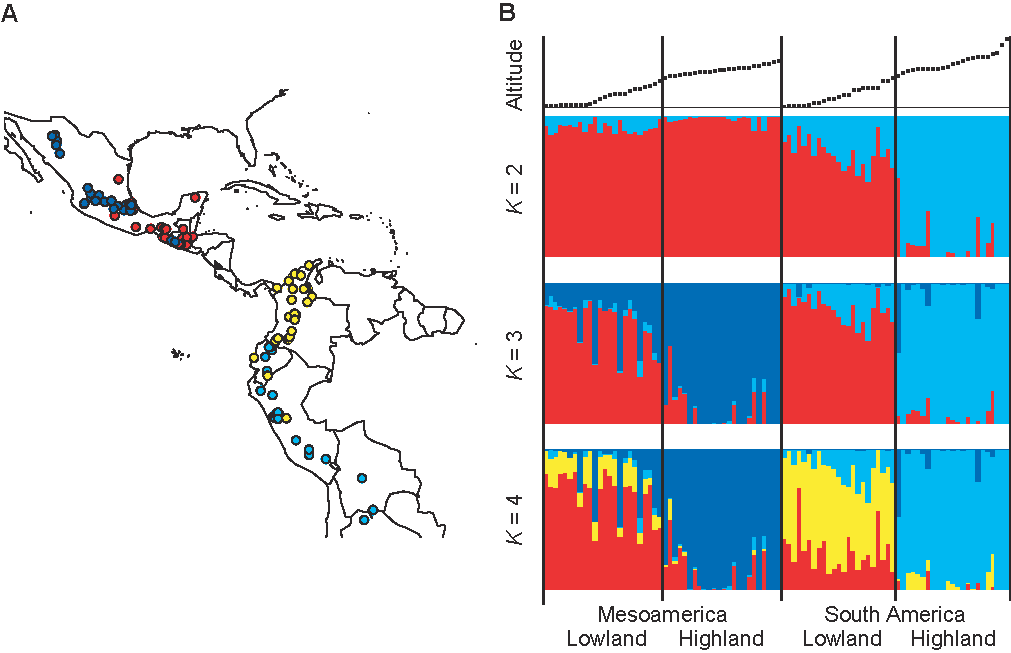
\includegraphics[width=0.8\textwidth]{fig/Fig2}
   \renewcommand{\baselinestretch}{0.9}
   \vspace{-3mm}
   \caption{(A) The sampling locations of landraces.  Red, blue, yellow and light blue dots represent Mexico lowland, Mexico highland, SA lowland and SA highland populations, respectively.  (B) The results of {\sf STRUCTURE} analysis with $K=2\sim4$.  The top panel shows the altitude of sampling locations of landraces, ranging from 0 to 4,000 m on the \emph{y}-axes.  The colors in $K=4$ correspond to those in panel (A).    }
\vspace{-6mm}
    \label{fig2}
  \end{center}
\end{figure*}
%%%%%%%%%%%%%%%%%%%%%%%%%%%%%%%%%%%%%%%%%% FIGURE

\section*{Materials and Methods}

\subsection*{Materials and DNA extraction}
We included 94 landraces (24, 24, 23 and 23 landraces sampled from Mexico lowland, Mexico highland, SA lowland and SA highland (Andean) populations).  These lines were provided by USDA and Major Goodman (supp Table S1).  Sampling locations are shown in Figure~\ref{fig2}A (see also supp table S1).   Lowland landraces were sampled from altitudes $<$1,700 m and highland landraces from  $>$1,700 m (supp table S1).  \comst{Matt, there is no information of the origin for some landraces (NA in supp table S1.  Do you have an idea?}  \mbh{I've saved a spreadsheet in the main folder of the dropbox with all the information I have on the accessions}Seeds were germinated on filter paper following fungicide treatment and grown in standard potting mix.  Leaf tips were harvested from plants at the five leaf stage.  Following storage at $-80{}^\circ$C overnight, leaf tips were lyophilized for 48 hours.  Tissue was then homogenized with a Mini-Beadbeater-8 (BioSpec Products, Inc., Bartlesville, OK, USA).  DNA was extracted using a modified CTAB protocol \cite[]{CTAB}.  The quality of DNA was ensured using methods described in \cite{vanHeerwaarden_2011_21189301}.

%Purity of extracted DNA was measured with a NanoDrop spectrophotometer (NanoDrop Technologies, Inc., Wilmington, DE, USA).  Samples with 260:280 ratios $\geq$1.8 were deemed acceptable for genotyping.  Concentrations of DNA extractions were determined with a Wallac VICTOR2 fluorescence plate reader (Perkin-Elmer Life and Analytical Sciences, Torrance, CA, USA) using the Quant-iT$^{TM}$ Picogreen(R) dsDNA Assay Kit (Invitrogen, Grand Island, NY, USA). \jri{we don't need to repeat all this, we can just cite van Heerwaarden 2012 PNAS or  Pyh\"aj\"arvi or Hufford (submitted) or maybe even Cook 2012 Plant Phys. for methods}

\subsection*{SNP data}
We used the maize B73 genome sequence RefGen version 2 as a reference \cite[]{Schnable_2009_19965430}.  
The filtered gene set (version 5b\_FGS) was retrieved from MaizeSequence.org for SNP annotations.  
We excluded transposable elements and pseudogenes from the filtered gene set. 
%\jri{we excluded TEs? TEs aren't in the FGS are they? What did you do to exclude these?}
%\comst{Jeff - there are 39249 protein coding genes, 323 pseudogenes and 84 transposable element in the FGS.} 
%\mbh{Sho, did you filter the FGS yourself for pseudogenes and TE's? If so, probably need to briefly describe your method.  If not, where did these annotations come from?  My understanding is these should be excluded from the FGS.}
Results were qualitatively similar when using the less stringently filtered working gene set (not shown).

We generated two complementary SNP data sets for the sampled maize landraces. 
The first set was generated using the Illumina MaizeSNP50 BeadChip platform, including 56,110
SNPs \cite[]{Ganal_2011_22174790}.  SNPs were clustered with the default algorithm of the GenomeStudio Genotyping Module v1.0 (Illumina Inc., San Diego, CA, USA).   
Clustering for each SNP was then visually inspected and manually adjusted.  
These data are referred to as "MaizeSNP50" hereafter.  
MaizeSNP50 data have high reproducibility and a low proportion of missing data but are subject to ascertainment bias. 
This array contains SNPs discovered in five ascertainment schemes \cite[]{Ganal_2011_22174790}; however, the vast majority of SNPs come from two panels: the Syngenta set (14,810 SNPs), derived from polymorphisms distinguishing the parents of the IBM mapping population (the maize lines B73 and Mo17), and the Panzea set, including 40,594 SNPs identified during sequencing of the 25 parents of the NAM mapping population.  
%\comst{numbers of panzea and syngenta SNPs will be added later}

The second data set was generated utilizing high-throughput Illumina sequencing data in a method referred to as \underline{g}enotyping-\underline{b}y-\underline{s}equencing (GBS).  \textcolor{red}{Kelly is up for details.}
Average coverage was relatively low \textcolor{red}{(5X?)} \jri{think more like 1X at best} resulting in heterozygotes often being miscalled as homozygotes.  However, this data set is relatively free from ascertainment bias.       
GBS data were obtained for a subset of 23, 23, 20 and 21 lines for Mexico lowland, Mexico highland, SA lowland and SA highland populations respectively (supp table S1).

%\subsection*{Quality of SNP data sets}

We compared SNP genotypes in the GBS and MaizeSNP50 data sets to assess data quality. 
Previous work has shown 2.45\% discordance in SNP genotypes between the maize HapMap2 data set and the MaizeSNP50 array. 
Most errors were due to mis-calling of heterozygous SNPs as homozygotes in the low coverage Hapmap2 data set \cite[]{Hufford_2012_22660546}. 
Our GBS data are also at low coverage which will likely result in an under-calling of heterozygotes.
We found that 7,197 SNPs overlapped between the MaizeSNP50 and GBS data sets. 
Excluding missing data, we compared 229,937 genotypes in the two data sets. 
While only 0.8\% of 173,670 homozygous loci in the MaizeSNP50 data set differed from GBS genotypes,
88.6\% of 56,267 MaizeSNP50 heterozygotes had different genotypes in the GBS data, being homozygous in nearly all cases. 
Despite an extremely high heterozygote error rate, our GBS data should be informative given the high correlation in allele frequencies between data sets ($r=0.89$; Supp fig. X) and a lack of major allele or reference bias (data not shown).


\subsection*{Structure analysis}
We performed {\sf STRUCTURE} analysis \cite[]{Pritchard_2000_10835412,Falush_2003_12930761} using  synonymous and noncoding SNPs from the MaizeSNP50 data. 
We assumed free recombination between SNPs without missing data and randomly pruned SNPs closer than 10 kb (alternative distances were tried with nearly identical results). 
Additionally, we removed SNPs showing an extreme excess of heterozygosity, a signal likely caused by paralogy. 
We also excluded SNPs in which the number of heterozygous individuals exceeded homozygotes and where the \emph{P}-value for departure from Hardy-Weinberg Equilibrium (HWE) based on a \emph{G}-test was smaller than 0.5\% using all individuals. 
Following these data thinning measures, 17,013 biallelic SNPs remained. 
We conducted three replicate runs of {\sf STRUCTURE} using the correlated allele frequency model with admixture for \emph{K} = 2$\sim$6 populations, a burn-in length of 50,000 iterations and a run length of 100,000 iterations. 
Results across replicates were nearly identical.
 

\subsection*{Inference of demography}

We tested three demographic models in which maize was differentiated into high- and lowland populations subsequent to domestication (Figure~\ref{model}). 
Observed joint frequency distributions (JFDs) were calculated using the GBS data set due to its lower level of ascertainment bias. 
A subset of silent SNPs were utilized that had $\geq15$ individuals without missing data in both low- and highland populations and did not violate HWE.  
An HWE cut-off of $P<0.005$ was used for each subpopulation due to our under-calling of heterozygotes. 
In total, we included 18,745 silent SNPs for the Mexican populations in Models I and II, 14,508 for the South American populations in Model I and 11,305 for the Mexican lowland population and the South American populations in Model III.  
We obtained similar results under more or less stringent thresholds for significance ($P < 0.05\sim0.0005$; data not shown), though the number of SNPs was very small when $P<0.05$.  
%\jri{not sure a reviewer will buy this.  the data are worse, so we are less stringent for HWE? I think we need to rephrase or rethink? are results similar if you use p<0.05?}  
Demographic parameters were inferred using the software {\sf dadi} \cite[]{Gutenkunst_2009_19851460}.  We calculated an expected JFD given parameters from a diffusion method and the likelihood obtained from the expected and observed JFDs in the multinomial approach of this software. \\


%%%%%%%%%%%%%%%%%%%%%%%%%%%%%%%%%%%%%%%%%% FIGURE
\begin{figure}[tb]   
  \begin{center}
   \vspace{-0mm}
   %\includegraphics[width=0.23\textwidth]{figs/model}
   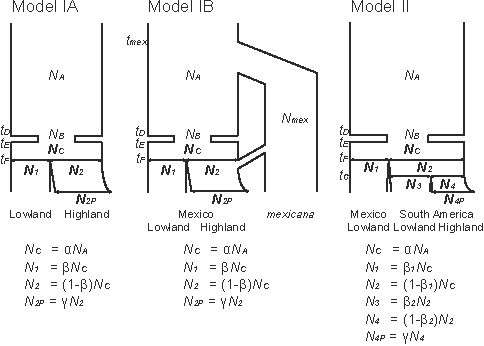
\includegraphics[width=0.5\textwidth]{fig/Fig3}
   \renewcommand{\baselinestretch}{0.9}
   \vspace{-3mm}
   \caption{Three demographic models of maize low- and highland populations.  Parameters provided in bold were estimated in this study.  See text for details.
   }
\vspace{-6mm}
    \label{model}
  \end{center}
\end{figure}
%%%%%%%%%%%%%%%%%%%%%%%%%%%%%%%%%%%%%%%%%% FIGURE

\subsubsection{Model I}
This model is applied to the Mexico and SA populations.
We assume the ancestral diploid population representing \emph{parviglumis} follows a standard Wright-Fisher model with constant size.  The size of the ancestral population is denoted by $N_A$.
At $t_D$ generations ago, the bottleneck event begins at domestication, and at $t_E$ generations ago, the bottleneck ends.  The population size and duration of bottleneck are denoted by $N_B$ and $t_B=t_D-t_E$, respectively.  The population size recovers to $N_C=\alpha N_A$ in the lowlands.  
Then, the highland population is differentiated from the lowland population at $t_F$ generations ago.  The size of the low- and highland populations at time $t_F$ is determined by a parameter, $\beta$ such that the population is divided by $\beta N_C$ and $(1-\beta)N_C$.  
We assume that, whereas the population size in the lowlands is constant, the highland population experiences exponential expansion after divergence: the current population size is $\gamma$ times larger than that at $t_F$.  \\

\subsubsection{Model II}
We expand Model I for the Mexico populations.  We incorporate admixture from \emph{mexicana} to the highland Mexican maize population.  The time of differentiation between \emph{parviglumis} and \emph{mexicana} occurs at $t_{mex}$ generations ago.  The size of the \emph{mexicana} population is denoted by $N_{mex}$ and this size is assumed to be constant.  At $t_F$ generations ago, the Mexico highland population is derived from the Mexico lowland population and admixture with \emph{mexicana}.  The proportion of admixture with \emph{mexicana} is denoted by $P_{mex}$.  \\

\subsubsection{Model III}
The final model is for the Mexico lowland, SA lowland and SA highland populations.  This model was used for simulating SNPs with ascertainment bias (see below).  At time $t_F$, the Mexico and SA lowland populations are differentiated, and the sizes of populations after splitting are determined by $\beta_1$.  At time $t_G$, SA lowland and highland populations are differentiated, and the sizes of populations at this time are determined by $\beta_2$.  As in Model I, the SA highland population is assumed to experience population growth with the parameter, $\gamma$.\\


%%%%%%%%%%%%%%%%%%%%%%%%%%%%%%%%%%%%%%%%%% FIGURE
\begin{figure}[tb]   
  \begin{center}
   \vspace{-0mm}
   %\includegraphics[width=0.23\textwidth]{figs/model}
   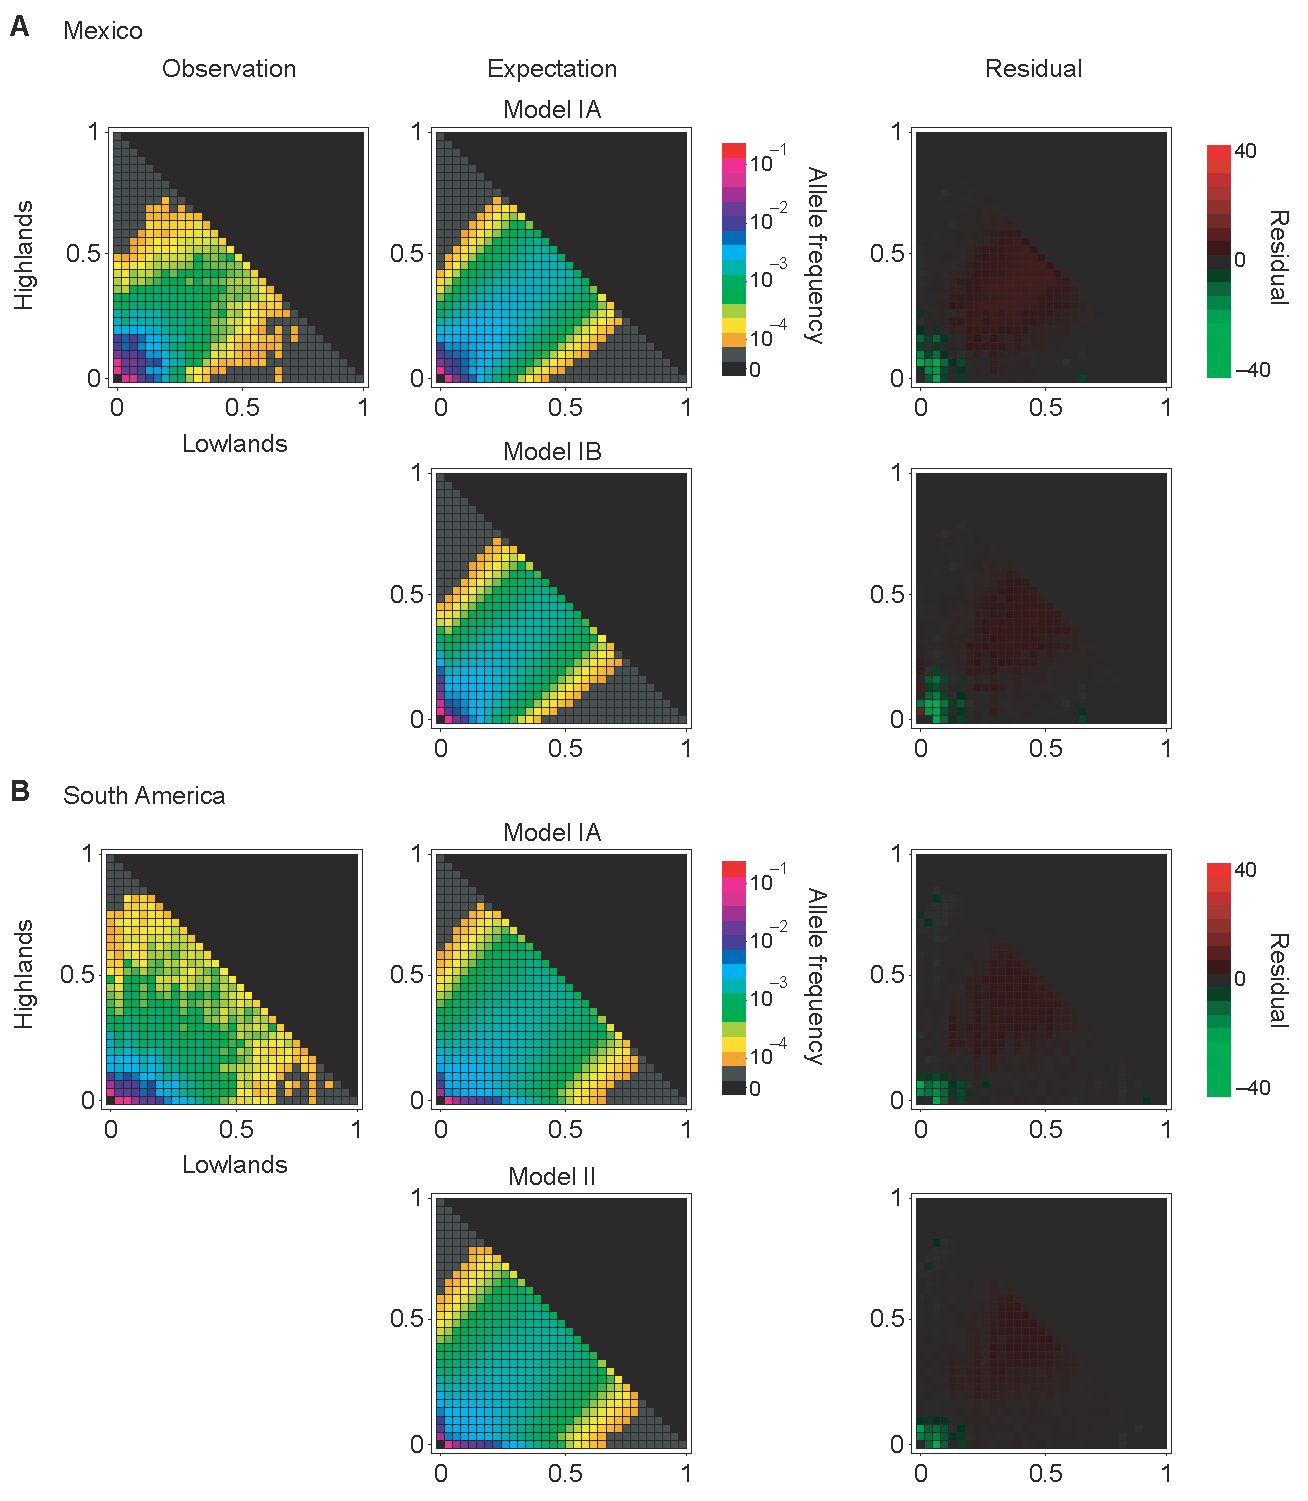
\includegraphics[width=0.5\textwidth]{fig/Fig4}
   \renewcommand{\baselinestretch}{0.9}
   \vspace{-3mm}
   \caption{Joined distributions of minor allele frequencies in low- and highland populations in (A) Mexico and (B) South America.  Observed JFDs, expected JFD and residuals are shown.  The scale bars of allele frequency and residual are also shown.     }
\vspace{-6mm}
    \label{JFD}
  \end{center}
\end{figure}
%%%%%%%%%%%%%%%%%%%%%%%%%%%%%%%%%%%%%%%%%% FIGURE

Several parameters in our demographic model were based on previous studies.  
$N_A$ was determined using estimates of the composite parameter $4N_A\mu$ and a separate estimate of mutation rate, $\mu$, per site per generation.  $4N_A\mu$ was estimated in \emph{parviglumis} to be $\sim$0.018  \cite[]{Eyre-Walker_1998_9539756,Tenaillon_2001_11470895,Tenaillon_2004_15014173,Wright_2005_15919994,Ross-Ibarra_2009_19153259}.  
The mutation rate in maize has been estimated to be $2.9\sim 3.3\times 10^{-8}$, so we assume $\mu=3\times 10^{-8}$ \cite[]{Clark_2005_16079248}.  
Thus, $N_A$ was set to $0.018/4/(3\times 10^{-8}) = 150,000$.
The severity of the domestication bottleneck is represented by $k=N_B/t_B$ \cite[]{Eyre-Walker_1998_9539756,Wright_2005_15919994}, and following \cite{Wright_2005_15919994}, we assumed $k=2.45$ and $t_B=1,000$ generations.  
Taking into account archaeological evidence \cite[]{Piperno_2009_19307570}, we assume $t_D=9,000$ and $t_E=8,000$.  
We further assumed $t_F=6,000$ for Mexican populations in Models I and II \cite[]{Piperno_2006_69}, $t_F=4,000$ for South American populations in Model I \cite[]{Perry_2006_16511492}, and $t_{mex}=60,000$, $N_{mex}=160,000$ \cite[]{Ross-Ibarra_2009_19153259}, and $P_{mex}=0.2$ \cite[]{vanHeerwaarden_2011_21189301} for Model II. 
Note that \cite{Profford_2013} recently estimated $P_{mex}=0.12$, \mbh{my overall estimate of $P_{mex}$ in STRUCTURE was $\sim$0.19, very similar to Joost's.  Estimates from HAPMIX were lower but were based on pretty ad hoc criteria} and we obtained very similar null distributions of $F_{ST}$ between Mexico low- and highland populations given $P_{mex}=0.1\sim0.2$.
Hereafter, we will show the result with  $P_{mex}=0.2$.
For both Models I and II, we inferred three parameters ($\alpha$, $\beta$ and $\gamma$), and, for Model III, we fixed $t_F=6,000$ and $t_G=4,000$ \cite[]{Piperno_2006_69,Perry_2006_16511492} and estimated the remaining four parameters ($\alpha$, $\beta_1$, $\beta_2$ and $\gamma$).

%We used GBS data for the observed JFDs because this data set is relatively free from ascertainment bias.  We screened silent SNPs with $\geq15$ individuals having no missing data in both low- and highland populations.  We further screened out SNPs departure from Hardy-Weinberg equilibrium.  Because of the low coverage of GBS data, a large proportion of heterozygotes were missed as shown above.  Thus, we used less strict cut-off, $P<0.005$ for each subpopulation.  In total, we used 18,745 silent SNPs for Mexico populations in Model I and II, 14,508 for SA populations in Model I and 11,305 for Mexico lowland population and SA populations in Model III.  When we used another cut-off such as $P<0.001$ or $P<0.0005$, we obtained similar estimations (not shown).  
 
\subsection*{Differentiation between low- and highland populations}
Based on inferred demography, we generated a null distribution of $F_{ST}$ by using {\sf ms} software \cite[]{Hudson_2002_11847089}.   
The command line options for {\sf ms} are provided in supp Table 2.  
For each combination of sample sizes in low- and highland populations, we generated $10^7$ $F_{ST}$ values given sample sizes and used these as a null distribution in order to evaluate our GBS data.   We calculated $F_{ST}$ values for all SNPs that had $\geq10$ individuals with no missing data in all four populations and showed no departure from HWE at the 0.5\% level. 

Calculation of differentiation using the MaizeSNP50 data is more complicated due to ascertainment bias.  
We addressed this problem by applying a simple method.  
The SNPs in this data set were discovered in a panel of maize inbred lines.  
These inbred lines appear to be derived from the Mexican lowland maize population based on examination of an NJ tree of inbred lines and our landrace samples constructed using our GBS data and SNPs in the Hapmap v2 data set \cite[]{Hufford_2012_22660546}. 
Therefore, we added two additional individuals to the Mexican lowland population and used only SNPs where the two individuals had different alleles.   
We used all SNPs where $\geq10$ individuals had no missing data in all four populations and where there was no departure from HWE at the 5\% level. As mentioned above, SNPs in this data set were discovered from multiple ascertainment schemes.  In the Results and Discussion, we demonstrate that the effect of different ascertainment schemes was not large.

\subsection*{Haplotype scoring test}
We performed a \underline{p}airwise \underline{h}aplotype \underline{s}coring (PHS) test to detect further evidence of selection, following \cite{Toomajian_2006_16623598}.  
To conduct this test, we first imputed and phased the combined SNP data (both GBS and MaizeSNP50) using the {\sf fastphase} software ver. 1.4.0 \cite[]{Scheet_2006_16532393}.  
As a reference for phasing, we used data (excluding heterozygous SNPs) from an Americas-wide sample of 23 partially inbred landraces that were included in the Hapmap v2 data set  \cite[]{Hufford_2012_22660546}.  
{\sf fastphase} was run with default parameter settings.  PHS was calculated for an allele \emph{A} at position $x$ by

\begin{equation}
  \label{phs-1}
  \begin{array}{l}
  \displaystyle{
PHS_{x_A} = \sum^{p-1}_{i=1}\sum^{p}_{j=i+1}Z_{ijx}  / \Bigl( \begin{array}{c} p \\ 2 \\ \end{array} \Bigr) 
- \sum^{n-1}_{i=1}\sum^{n}_{j=i+1}Z_{ijx}  / \Bigl( \begin{array}{c} n \\ 2 \\ \end{array} \Bigr) 
  }
  \end {array} 
  \textrm{,}
\end{equation}

\noindent where $n$ is sample size of haploids, $p$  is the number of haploids carrying the allele $A$ at position $x$, and

\begin{equation}
  \label{phs-2}
  \begin{array}{l}
  \displaystyle{
Z_{ijx} = \frac{ d_{ijx} - \bar{d_{ij}} }{ \sigma_{ij} }
  }
  \end {array} 
  \textrm{,}
\end{equation}

\noindent where $d_{ijx}$ is the genetic distance over which individuals $i$ and $j$ are identical surrounding position $x$, $\bar{d_{ij}}$ is the genome-wide mean of distances over which individuals are identical, and $\sigma_{ij}$ is the standard deviation of the distribution of distances.  
The \emph{P}-value for an allele $A$ with frequency $p$ at position $x$ was calculated such that Pr($PHA_{xA}\leq PHA_{null|p}$), where $PHA_{null|p}$ are the PHS values for all alleles with frequency $p$ across the genome. 
%\mbh{so is $PHA_{p}$ a mean?}
%\mbh{The previous sentence needs to be clarified}

Genetic distances were obtained from the IBM mapping population \cite[]{Ganal_2011_22174790}.  
While genetic positions were initially only available for the MaizeSNP50 data set, we fit genetic (cM) and physical (bp) distances to a tenth degree polynomial curve, and calculated cM for all SNPs. 
%\jri{ should we provide this data online or in supp.? not sure}
%\comst{you mean PHS?}
 
%%%%%%%%%%%%%%%%%%%%%%%%%%%%%%%%%%%%%%%%%% FIGURE
\begin{figure}[tb]   
  \begin{center}
   \vspace{-0mm}
   %\includegraphics[width=0.23\textwidth]{figs/model}
   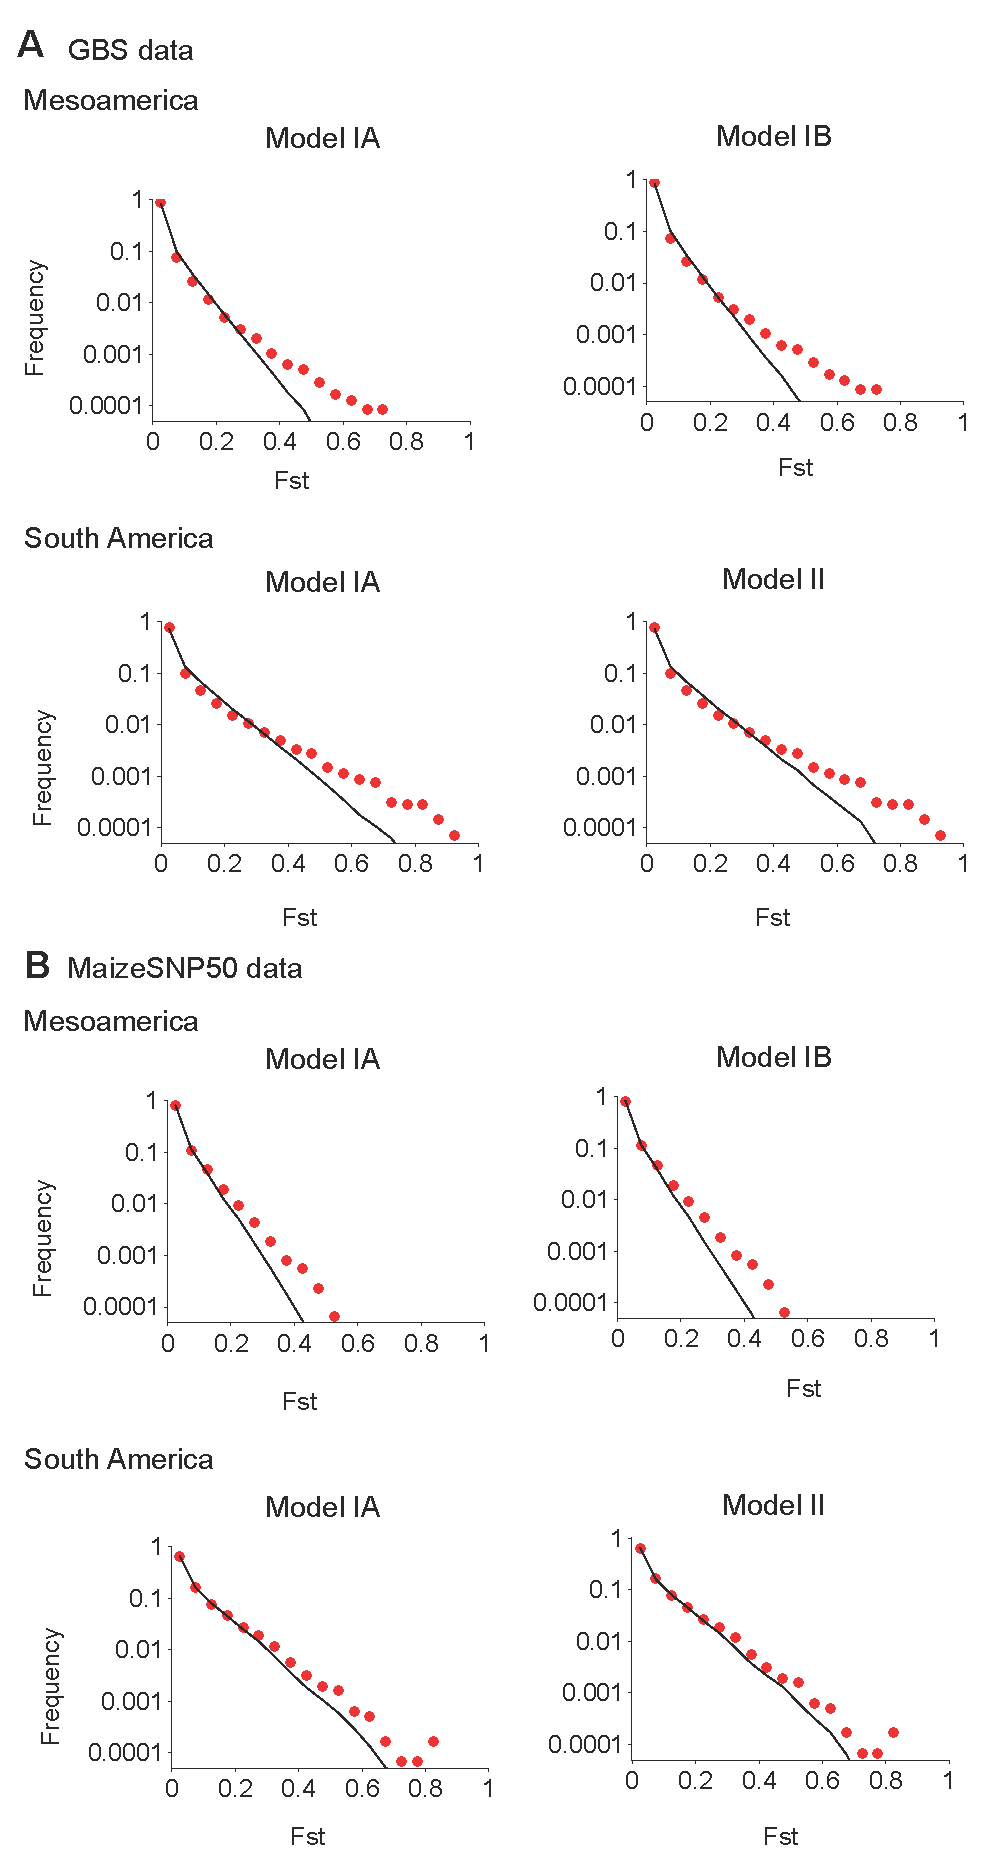
\includegraphics[width=0.45\textwidth]{fig/Fig5}
   \renewcommand{\baselinestretch}{0.9}
   \vspace{-3mm}
   \caption{Observed and expected distributions of $F_{ST}$ values in GBS (A) and MaizeSNP50 data (B).  \The \emph{x}-axes represent $F_{ST}$ values.  The \emph{y}-axes represent the frequency of SNPs with $F_{ST}$ values within a bin of 0.05 size.  Red dots and solid lines indicate observed and expected distributions. %\jri{this is cumulative proportion of SNPs?  not sure what "frequency" on y axis means" }\comst{clarified.  Maybe I shouldn't use solid lines.  Thoughts? }
   }
\vspace{-6mm}
    \label{FstDist}
  \end{center}
\end{figure}
%%%%%%%%%%%%%%%%%%%%%%%%%%%%%%%%%%%%%%%%%% FIGURE


%%%% PLR:
\subsection*{Migration and new mutation of adaptive alleles}

We suggest below that many of these high-$F_{ST}$ alleles are locally adaptive,
and the degree of coincidence between highland regions informs us about 
whether these adaptations occurred indpendently (in parallel), or if alleles transited between the two.
To see if the abundance and degree of coincidence is consistent with what is known about the population history of maize,
we evaluated the rate at which we expect an allele that provides a selective advantage at higher altitude
to arise by new mutation in a highland region ($\mutrate$),
and the rate at which such an allele already present in the Mexican highlands
would transit the intervening lowlands and fix in the Andean highlands ($\migrate$),
in both cases assuming it is slightly deleterious at lower altitude.
These numbers depend most strongly on the population density, 
the selection coefficient,
and the rate at which seed is transported long distances and replanted.
We evaluated these rates using new and existing theory, and validated by simulation.

\plr{
A note here on why we assume it is deleterious?  
It would be possible to say convincing things about the case where it is neutral at low elevation,
but will require significant thinking (which I've begun to do\dots).
}

To calculate the rate at which new mutations appear and fix in the highland population, $\mutrate$,
we simply used the total population size of the highlands
multiplied by the mutation rate per generation
and by the chance that a single such mutation successfully fixes
(i.e.\ is not lost to drift).
The latter probability, that a single new mutant allele providing benefit $s_b$ to heterozygotes at high elevation
will increase in frequency and fix in the high elevation patch,
is approximately $2s_b$ divided by the variance in offspring number \citep{jagers1975branching}.
This is not quite right, since such a mutation could occur at low elevation,
where it is deleterious,
and its offspring could then migrate to high elevation and fix there.
Similarly, if we use the selection coefficient for high elevation,
this ignores the fact that some of the seeds from the high-elevation plants may be grown at low elevation,
reducing the chance of fixation of an allele that appears at high elevation.
This scenario has been well-studied in theoretical models by \citet{polk} and \citet{barton1987establishment},
% missing reference for Polk.
but it is not immediately obvious how well their approximations apply to maize,
as it grows across an altitudinal gradient (rather than an abrupt transition) and has high variance in number of offspring.
Therefore, we used the following more detailed demographic model (following \citet{vanHeerwaarden2010}) 
%cite van Heerwaarden  2010 Heredity
to numerically calculate the chance of fixation of a beneficial allele
as a function of the location it first appears.
We found that the simple approximation is quite good,
although the demographic model was necessary to find the variance in offspring number,
as well as the migration rate, which we will need later.

TODO: describe demographic model in words.  (including migration which we need later.)
Reference math and more detail in appendix.

\plr{could alternatively: (a) describe the math; or (b) cut this down further.}

Concretely, the probability that a new mutation destined for fixation
will arise in a patch of high-elevation habitat of area $A$ in a given generation
is a function of the density of maize per unit area $\rho$,
the selective benefit $s_b$ it provides,
the mutation rate $\mu$,
and the variance in offspring number $\xi^2$.
In terms of these parameters, the rate of appearance is
\begin{align} \label{eqn:mutrate}
  \mutrate = \frac{2 \mu \rho A s_b}{\xi^2} .
\end{align}

A corresponding expression for the chance that an allele moves from one highland population to another is harder to intuit,
and is addressed in more depth in \citep{ralphcoop2013patches}.
If an allele is beneficial at high elevation, and fixed in the Mexican highlands,
but deleterious at low elevations,
then it will be present at low frequency in nearby lowland populations,
maintained at migration-selection balance \citep{slatkin1973geneflow}.
(Here ``migration'' is mediated by farmer exchange of seed stocks.)
This equilibrium frequency decays exponentially with distance,
so that the highland allele is present at distance $R$ from the highlands at frequency $C \exp(- R \sqrt{2s_m} / \sigma)$,
where $s_m$ is the deleterious selection coefficient for the allele in low elevation,
$\sigma$ is the mean dispersal distance (mean distance between parent and offspring),
and $C$ is a constant depending on geography ($C\approx 1/2$ is close).
Multiplying this frequency by a population size gets the predicted number of individuals carrying the allele in that population,
which at large distances can be less than 1;
this is possible because this is the average density of selected alleles across a large number of generations.
Therefore, in a lowland population of size $N$ at distance $R$ from the highlands,
$(N/2)  \exp(- R \sqrt{2s_m} / \sigma)$ is equal to the probability that there are any highland alleles present,
multiplied by the expected number of these, given that there are some present.
Since the latter is at least 1,
the chance there are any present in a given generation is no more than $(N/2) \exp(- R \sqrt{2s_m} / \sigma)$,
and so this puts an upper bound on $\migrate$.
Therefore, we would need to wait around $\Tmig = (2/N)\exp(R \sqrt{2s_m} / \sigma)$ generations 
for a rare such excursion to occur.
Concretely, we can use that
\begin{align}
  \migrate \le (N/2)  \exp(- R \sqrt{2s_m} / \sigma) ,
\end{align}
with $N$ the total size of the unadapted highland population,
and $R$ the distance from the adapted to the yet-undapted highland populations.
Another factor this omits is the probability that such an allele fixes;
however, since such alleles arrive by migration, which are planted out into a field,
it is not too bad, and conservative, to neglect the factor of $2s_b/\xi^2$,
if we count $N$ as the number of \emph{parent} plants used to replant the region each year.

To obtain specific predictions,
we then computed $\mutrate$ and $\migrate$ at various paramter values.
We also checked these with simulations and more detailed computations,
described in the Appendix.
\plr{I am flexible about what goes in that appendix\dots}


\section*{Results and Discussion}


%%%%%%%%%%%%%%%%%%%%%%%%%%%%%%%%%%%%%%%%%%%%%%%%%%%%%%%%%%%%
\renewcommand{\arraystretch}{1.1}
\begin{table}[tb]

\begin{center}
 \caption[]{Pairwise $F_{ST}$ among populations \hspace*{2.3cm}}
  \textbf{}\\[-2mm]
{\fontsize{7}{9}\sf
    \begin{tabular}{llccccccl}
    \hline
    & & \\[-3mm]
	&		&	\multicolumn{2}{c}{Mexico}		&	\multicolumn{2}{c}{South America}		\\
	&		&	Lowlands	&	Highlands	&	Lowlands	&	Highlands	\\
      \hline
    & & \\[-3mm]
Mexico	&	Lowlands	&	--	&		&		&		\\
	&	Highlands	&	0.0244	&	--	&		&		\\
SA	&	Lowlands	&	0.0227	&	0.0343	&	--	&		\\
	&	Highlands	&	0.0466	&	0.0534	&	0.0442	&	--	\\ [1mm]
    \hline
	\multicolumn{6}{l}{SNPs from GBS data were used with $2n\geq20$ for each population.}

    %\jri{mention from what data}
%    \multicolumn{9}{l}{$^{a}$ The groups were based on phylogenetic analysis in fig.~\ref{tree}\emph{A}}\\
    \end{tabular}
    \label{FstP}  % caption is needed to make this work
}
\end{center}
\end{table}
\renewcommand{\arraystretch}{1}
%%%%%%%%%%%%%%%%%%%%%%%%%%%%%%%%%%%%%%%%%%%%%%%%%%%%%%%%%%%%

\subsection*{Population structure}

We performed a {\sf STRUCTURE} analysis  \cite[]{Pritchard_2000_10835412,Falush_2003_12930761} 
using MaizeSNP50 data due to its lower error rate for genotyping heterozygotes. 
Accurate estimates of allele frequencies are necessary for this analysis because populations are inferred by minimizing deviations from HWE.
The number of groups was varied from $K=2\sim6$ and the likelihood given $K$ reached a plateau at $K=3$ (Supp FigX).
Several observations can be made based on results from $K=2\sim4$. 
First, most landraces were assigned to groups consistent with our \emph{a priori} population definitions.
Second, while admixture between highland and lowland groups was apparent at intermediate elevations ($\sim1700$m) in both Mexico and South America, greater highland/lowland differentiation was observed in South America.  
Strong divergence of South American highland landraces was supported by their relatively high level of differentiation ($F_{ST}$) from other populations at noncoding and synonymous sites in the GBS data set and may be indicative of a strong bottleneck during colonization of this region.
Third, the Mexican lowland population shared ancestry with both the Mexican highland and South American lowland populations, consistent with a previously described scenario for maize diffusion \cite[]{Piperno_2006_69}.  
Finally, Mexican and South American highland landraces were consistently assigned to separate groups suggesting strong differentiation between maize in these regions.

%\jri{ testing to see if model is robust to amount of gene flow might be easy to do?}
%\comst{check fst with $P_{mex} = 10\%$!!}

%{\sf STRUCTURE} results in Fig.~\ref{fig2}B suggest the level of divergence between low- and highland populations may be higher in South America than in Mexico.
%We next calculated average $F_{ST}$ values among populations at noncoding and synonymous sites from GBS data ($2n\geq20$ for each population; Table~\ref{FstP}).
%Consistent with the results of {\sf STRUCTURE}, the South American highland population showed a relatively high level of differentiation from the other populations.
%\jri{why silent? i don't see it used much anymore, i think because people have enough data that they can separate out synonymous... thoughts?}
%\st{When using only noncoding SNPs, we obtained almost the same result.
%When using only synonymous SNPs, $F_{ST}$ values became slightly smaller (not shown or supp?). Finally, when using non-synonymous SNPs, Fst decreased even further.}
%The JFD calculated from silent sites of GBS data ($2n\geq30$ for each population) showed a similar trend.  Moreover, as is apparent in Figure ~\ref{JFD}, the variance of change in allele frequency between low- and highland populations is much larger in South America than in Mexico.
%Archaeological evidence suggests that population divergence occurred more recently in South America  \cite[]{Piperno_2006_69,Perry_2006_16511492,Grobman_2012_22307642}.  Combined these factors suggest that the South American highland population may have experienced a stronger bottleneck than the Mexican highland population.
 
 %%%%%%%%%%%%%%%%%%%%%%%%%%%%%%%%%%%%%%%%%%%%%%%%%%%%%%%%%%%%
\renewcommand{\arraystretch}{1.1}
\begin{table}[tb]

\begin{center}
 \caption[]{Inference of demographic parameters\hspace*{0.3cm}}
  \textbf{}\\[-2mm]
{\fontsize{7}{11}\sf
    \begin{tabular}{lcccccccl} \hline
       & & \\[-3mm]
     Mexico  & \multicolumn{2}{c}{Model I}  &\multicolumn{2}{c}{Model II}\\[0.1cm]
    \hline
    & & \\[-3mm]
   & Likelihood & $-$5590.33 & Likelihood &  $-$4641.28 \\
  &$\alpha$    & 0.92  & $\alpha$    & 1.5 \\
  &$\beta$ & 0.38  & $\beta$  & 0.75\\ 
  &$\gamma$   & 1        &  $\gamma$   & 1\\ 
      \hline
    & & \\[-3mm]
    South America  & \multicolumn{2}{c}{Model I}  &\multicolumn{2}{c}{Model III}\\[0.1cm]
        \hline
    & & \\[-3mm]
     & Likelihood &  $-$3858.48 & Likelihood &  $-$8016.88 \\
      &$\alpha$    & 0.55           & $\alpha$       & 1.0 \\
      &$\beta$ & 0.97           & $\beta_1$   & 0.64\\ 
      &$\gamma$   & $\geq$60   &  $\beta_2$  & 0.95\\ 
      &                &                     &  $\gamma$       & $\geq$55\\ [1mm]
    \hline
%    \multicolumn{9}{l}{$^{a}$ The groups were based on phylogenetic analysis in fig.~\ref{tree}\emph{A}}\\
    \end{tabular}
    \label{param}  % caption is needed to make this work
}
\end{center}
\end{table}
\renewcommand{\arraystretch}{1}
%%%%%%%%%%%%%%%%%%%%%%%%%%%%%%%%%%%%%%%%%%%%%%%%%%%%%%%%%%%%
% When P_mex=0.1, alpha=1.1, beta = 0.67



\subsection*{Population differentiation under inferred demography}

Demographic parameters were estimated for lowland and highland populations in both Mexico and South America in order to provide a neutral expectation for population differentiation.  
Models were fit (Fig.~\ref{model}) to the observed JFDs using the maximum likelihood method implemented in {\sf dadi} \cite[]{Gutenkunst_2009_19851460}.  
Estimated parameters are listed in Table~\ref{param} and expected JFDs and residuals are shown in Fig.~\ref{JFD}.  
Overall, the observed and expected JFDs were similar in the two models in both Mexico and South America.
However, residuals indicated an excess of rare variants in the observed JFDs in all cases.  We demonstrate below that this factor should not greatly affect our analysis of population differentiation.

Under both Models I and II In Mexico, we found expansion in the highland population to be unlikely.  
The likelihood value of Model lI ($-$4641.28) was much higher than the likelihood of Model I ($-$5590.33) (Table~\ref{param}), providing evidence that introgression from \emph{mexicana} may have been an important factor during the spread of maize into the Mexican highlands. \mbh{It may be worth running an AIC test on these two models to see if the addition of an introgression parameter significantly improves the likelihood}%However, expected JFDs are visually similar. 
%\jri{i have a bit of trouble understanding this.  if the likelihood is much higher, why would the JFDs be identical?  or does "similar" simply mean in some gross overall sense?}  
%\comst{Jeff - JFDs are not identical, though they look identical. } 
A very strong bottleneck followed by population expansion is supported in maize from the South American highlands based on parameterization of Models I and III.  

\subsubsection{GBS data}We identified significantly differentiated SNPs between low- and highland populations by comparing our empirical $F_{ST}$ values to the neutral expectation given inferred demography.
We simulated $10^7$ SNPs using {\sf ms} software \cite[]{Hudson_2002_11847089} and our inferred demographic parameters and calculated \emph{P}-values for population differentiation in our empirical data using simulated $F_{ST}$ values as a null distribution.  
Two parameter sets were employed for both Mexico (Model I and II) and South America (Model I and III) (Table~\ref{param}).
Model choice had little effect in both Mexico and South America (\emph{i.e.,} we obtained very similar null distributions of $F_{ST}$ values (Figure~\ref{FstDist}A)).
Moreover, null and observed distributions of $F_{ST}$ values were quite similar under our tested models (Figure~\ref{FstDist}A).
Thus, although we observed an excess of rare variants in the observed JFDs (Figure~\ref{JFD}), our results should be conservative.

We also tested the robustness of our analysis of population differentiation to the specification of the model.  
%The distributions of calculated \emph{P}-values were also similar between the models both in Mexico and South America (Supp Figure~4).
In addition to the parameters listed in Fig.~\ref{model}, we treated the size of the domestication bottleneck  ($N_B$) as a variable parameter.  
Surprisingly, $N_B$ was estimated to be equal to the population size at the end of the bottleneck, $N_C$ (\emph{i.e.,} no bottleneck was most likely; supp Table~3).  
Moreover, the likelihood was much smaller for a bottleneck model (supp table~3) than for alternative models described in Table~\ref{param}, suggesting a domestication bottleneck did not occur.
This result may at first seem surprising given previous work regarding the demography of maize during domestication.  For example, \cite{Wright_2005_15919994} inferred the strength of the domestication bottleneck by analyzing coding regions and found these to have an excess of SNPs with intermediate allele frequencies, a population signature consistent with a recent bottleneck.  
In contrast, \cite{Hufford_2012_22660546} demonstrated that intergenic regions in maize, unlike coding regions, showed an excess of rare variants.
Our JFDs using SNPs from across the genome (\emph{i.e.}, both genic and intergenic) also showed an excess of rare variants from the expectation under \cite{Wright_2005_15919994}'s bottleneck model.
%Higher density data may be necessary to adequately infer the domestication bottleneck.
The effects of the maize domestication bottleneck may therefore be most apparent in coding regions.
 Nevertheless, presence versus absence of a bottleneck had little effect on distributions of \emph{P}-values for differentiation between highland and lowland maize as shown in supp figure~5.  %, though \emph{P}-values became a bit bigger without the bottleneck. 
%\mbh{what is meant by bigger p-value? More significant (i.e., smaller value)?  Is this really negligible?  Not sure it's necessary to tag this on to the end.}  
 
%\st{Need to explain why?  Stephen used coding regions, but we use SNPs from whole genome.    Oh, this is beyond the scope of our paper!!} \jri{no this is a cool result that needs to stay in the discussion}


\subsubsection{MaizeSNP50 data}To overcome ascertainment bias in the MaizeSNP50 data set, we employed a simple method in which we added two individuals to the Mexican lowland population representing the maize lines B73 and Mo17. For Model I in South America we added two individuals at time $t_F$ to the ancestral population of the South American low- and highland populations because the Mexican lowland population was not incorporated into this model.  Without this modification of our demographic model, we underestimated \emph{P}-values, but the effect was very small (Supp Figure~6).   Furthermore, the empirical and null distributions of $F_{ST}$ values were very similar in the MaizeSNP50 data set despite the fact that multiple ascertainment schemes were used (Figure~\ref{FstDist}B; Supp Figure~6). 

%%%%%%%%%%%%%%%%%%%%%%%%%%%%%%%%%%%%%%%%%% FIGURE
\begin{figure}[tb]   
  \begin{center}
   \vspace{-0mm}
   %\includegraphics[width=0.23\textwidth]{figs/model}
   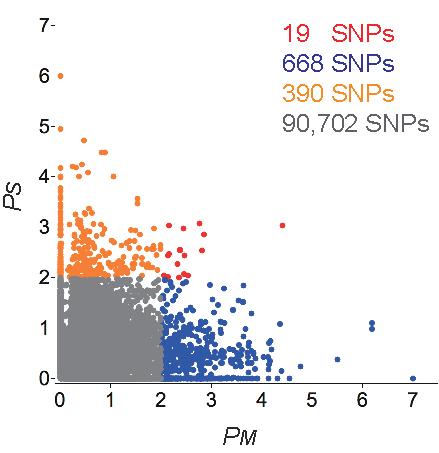
\includegraphics[width=0.4\textwidth]{fig/Fig6}
   \renewcommand{\baselinestretch}{0.9}
   \vspace{-3mm}
   \caption{Scatter plot for \emph{P}-values of population differentiation between low- and highland populations in Mexico ($P_X$ on \emph{x}-axes) and South America ($P_S$ on \emph{y}-axes).  $P_M$ and $P_S$ are scaled by --log$_{10}$.  Red, blue, orange and gray dots represents SNPs showing significance in both Mexico and South America, only in Mexico, only in South America, respectively.} \jri{do we know what that clear outlier red SNP is? anything interesting?}
\vspace{-6mm}
    \label{PvDist}
  \end{center}
\end{figure}
%%%%%%%%%%%%%%%%%%%%%%%%%%%%%%%%%%%%%%%%%% FIGURE




\subsubsection{Joint data set}In total, 91,779 SNPs remained in our joint, filtered GBS and MaizeSNP50 data set ($2n\geq20$ and HWE $P\geq0.005$ \mbh{need to keep track of how this is reported: sometimes 0.005, sometimes 0.5\%} for GBS or $P\geq0.05$ for MaizeSNP50 for all four populations).  For the Mexican and South American populations, we calculated \emph{P}-values for 76,989 and 63,160 SNPs respectively with the remaining SNPs being monomorphic. The reduced number of polymorphic SNPs in South America relative to Mexico is likely due to a lower effective population size in the South American populations.  48,370 SNPs were polymorphic in both Mexico and South America. 


We chose $P<0.01$ as an arbitrary cut-off for significant differentiation between low- and highland populations.  
We found 1,040 SNPs with $P<0.01$ in Mexico (1,040/76,989=0.0135) and 756 in South America (756/63,160=0.0120).  
Expected and observed numbers of significance were almost equal.  
In total, 1,740 SNPs showed significant differentiation in Mexico and/or South America.

\subsection*{Patterns of adaptation}

\subsubsection{Adaptation via mutation versus standing variation}

In order to characterize patterns of adaptation we first determined whether putatively adaptive variants (\emph{i.e.}, highly differentiated SNPs between the lowlands and the highlands) arose primarily through new mutations or standing genetic variation.  
We found that putatively adaptive variants in both Mexico and South America tended to segregate in lowland populations more commonly than the remainder of SNPs (84.6\% vs. 74.8\% in Mexico, FET {$P < 10^{-11}$ and 87.3\% vs 81.8\% in South America,  $P< 10^{-3}$).  
\plr{What does ``adaptive variants tended to segregate'' mean?  That high $F_{ST}$ SNPs are more likely to be polymorphic in those pops?}
We extended this analysis to standing variation in \emph{parviglumis}, the progenitor of domesticated maize, by retrieving genome-wide SNP data from 14 \emph{parviglumis} inbred lines included in the Hapmap v2 data set, using only SNPs with $n\geq10$ \cite[]{Hufford_2012_22660546}.  Again we found that putatively adaptive variants tended to segregate to a disproportionate extent in \emph{parviglumis} (81.1\% vs. 72.1\% in Mexico, FET {$P < 10^{-6}$ and 81.2\% vs 72.7\% in South America,  $P< 10^{-4}$).  \mbh{Sho, I extensively edited the previous sentences of this paragraph.  I was careful to keep all \%'s and $P$-values straight, but might be a good idea to double check} 

\textcolor{red}{It has been demonstrated that the domestication traits in maize were mainly established such that the frequency of maize-type alleles was increased that are maintained at low frequency in teosinte.  \emph{tb1} (who reported this first?) and \emph{gt1} \cite[]{Wills_arXiv} are, for example, the case (and more?).  Our results may extend this view: selection from standing variation are mainly involved in the processes of domestication and local adaptation in maize.  
Recently, the lines of evidence for selection from standing variation is increased in model organisms such as Drosophila (Petrov arXiv) and human \cite[]{Turchin_2012_22902787,Peter_2012_23071458}.}

%compare to above
%\textcolor{red}{It has been demonstrated that the domestication traits in maize were mainly established such that the frequency of maize-type alleles was increased that are maintained at low frequency in teosinte.
%\emph{tb1} \cite[]{Studer_2011_21946354}, \emph{ba1} \cite[]{Gallavotti_2004_15577912}, \emph{ra1} \cite[]{Sigmon_2010_20196812} and \emph{gt1} \cite[]{Wills_arXiv} are, for example, the case.  Our results may extend this view: selection from standing variation are mainly involved in the processes of domestication and local adaptation in maize.


In summary, the progenitor populations of highland maize (lowland maize and \emph{parviglumis}) contain both genotypes of highly differentiated SNPs implying adaptation from standing variation.
However, standing variation may be difficult to distinguish from gene flow between lowland and highland populations due to their recent divergence in units of $N_A$.
An additional caveat is that our inference of adaptation from standing variation assumes that our highly differentiated SNPs are causal and not merely linked to the targets of adaptation.  A causal variant at some distance from the assayed SNP may have had the opportunity to recombine onto multiple backgrounds. 
%I think we can drop this explanation? The more likely one is that we missed stuff entirely, no?
Given the previously documented rapid decay of linkage disequilibrium in maize \cite[]{Tenaillon_2001_11470895,Remington_2001_11562485} that is also apparent in our data (supp fig.~X) we are also likely missing a number of selected loci not in LD with the SNPs assayed here.

\mbh{Please note that I've commented out a large amount of text and comments at this point in the manuscript.  Probably a good idea to read through this to make sure there are not parts that you would like to bring back.}

%\st{(Or we can say without gene flow, we can well explain the observed pattern of polymorphisms).
%Lots of shared polymorphisms between maize and teosinte may support the standing variation hypo? Standing variation hypo holds as long as the effect of gene flow between maize and teosinte is negligible. 
%In fact, \cite{vanHeerwaarden_2011_21189301} estimated admixture between Mexico lowlands maize and \emph{parviglumis} to be very low. 
%Admixture from  \emph{parviglumis} to maize may alter the shape of the null distributions of $F_{ST}$ values.
%We checked even high admixture (up to 20\%) did not change the distributions (\cite{vanHeerwaarden_2011_21189301} estimated a few percentage of admixture).
%Thus, our $F_{ST}$ outlier approach is conservative on gene flow.}

\subsubsection{Highland versus lowland adaptation}

Given the history of the spread of maize, it is tempting to assume that significant population differentiation is due to an increase in frequency of adaptive alleles in the highlands.
However, we cannot rule out the possibility of adaptation in the lowlands.
Therefore we further investigated patterns of allele frequency change across populations.
When data were available for \emph{parviglumis} from Hapmap v2 \cite[]{Chia_2012_22660545,Hufford_2012_22660546}, we included these in our analysis.

First, we assessed patterns of allele frequencies in SNPs that were significantly differentiated between highland and lowland maize.
We focused on SNPs segregating as shown in Fig.~\ref{tes2}A, although some SNPs showed more complex patterns.
The first and second rows show hypothesized patterns of segregation under highland adaptation; here, allele frequencies in maize from a highland region are highly differentiated from those of \emph{parviglumis} and maize from the corresponding lowland region. %and no difference is observed between South America populations.
%When \emph{parviglumis} data are lacking, SNPs showing the pattern of segregation in the third row likely underly highland adaptation.
%\mbh{don't think this row in the figure is necessary}
Similarly, patterns of SNP segregation depicted in the fourth to sixth rows are consistent with lowland adaptation.
%The patterns expected for highland and lowland adaptation in South America are qualitatively the same as those shown for Mexico in Fig.~\ref{tes2}A.
We found that 74.5\% (400/537) and 84.5\%(448/530) of putatively adaptive SNPs in Mexico and South America respectively that displayed segregation patterns consistent with highland adaptation also had lower P-values for the PHS test in highland maize.
Likewise, 63.5\% and 67.1\% of the putatively adaptive SNPs in Mexico and South America that showed segregation patterns consistent with lowland adaptation also showed lower P-values for the PHS test in lowland maize.
Additionally, when a putatively derived allele segregated in both the lowlands and highlands but was more prevalent in the highlands, 67.5\% and 67.6\% of such SNPs showed lower PHS \emph{P}-values in the highlands in Mexico and South America. 
\jri{is this more that show the PHS stat than expected? that is if you pick random alleles, or maybe random alleles at similar frequencies?}
\comst{I tested: $P<10^{-11}, < 0.01$, $\approx 0$, $<10^{-9}$ for Mex high, Mex low, SA high and SA low, respectively}


\subsubsection{Adaptation through introgression}

 A marked difference between highland adaptation of maize in Mexico and South America is the potential for adaptation through introgression from wild relatives.  While maize in Mexico grows in sympatry with both the lowland taxon \emph{parviglumis} and the highland taxon \emph{mexicana}, maize in South America is outside the range of the wild \emph{Zea} species.
 \cite{Tanja_arXiv} recently assessed the potential for local adaptation in \emph{parviglumis} and \emph{mexicana} populations, characterizing differentiation between these subspecies using an Fst-outlier approach.
%\emph{parviglumis} and \emph{mexicana} inhabit the Mexico lowlands and highlands, respectively, so we expected that some some SNPs highly differentiated between these subspecies would overlap highly differentiated SNPs lowland and highland Mexican maize.
We observed a significant excess of overlap between our putatively adaptive SNPs in Mexican maize and those identified in the \cite{Tanja_arXiv} analysis (Table~\ref{tanja}; $P<0.01$ by FET).
Significant overlap was also observed with South American maize populations ($P<0.01$), but the proportion of SNPs was lower than observed in Mexico.  These data suggest that adaptations in Mexican maize may have been obtained through gene flow with wild relatives.  To more fully explore this hypothesis we evaluated our data in light of introgression identified by \cite{Profford_2013} from \emph{mexicana} into maize in the Mexico highlands.  
The proportion of significant SNPs in introgressed regions in Mexico is significantly higher than found in South America (Fisher's exact test, $P\ll0.001$).
%When focusing on GUs, we identified 99/586 (14.5\%) and 22/466 (4.7\%) GUs of Mexico- and SA-specific significance in introgressed regions (Fisher's exact test, $P<10^{-6}$). 
\plr{This part is very nice.  I did wonder how different the proportions are?}
Outside introgressed regions, the Mexican and South American populations did not show marked differences in the proportion of significant SNPs (Fisher's exact test, $P>0.7$). %\jri{cool!}  
These trends indicate \emph{mexicana} has played a more substantial role in conferring highland adaptation to maize in Mexico than in South America as would be expected considering the range of \emph{mexicana} does not extend to South America.

\textcolor{red}{One more thing.  The SNPs with significant $F_{ST}$ $P$-values are enriched in intergenic regions than ones with non-significant $P$-values (51.3\% vs. 44.2\%; FET $P < 10^{-8}$).  That would be consistent with the idea that selection on regulatory regions is a predominant force in the maize domestication process (Doebley?). On the other hand, the comparison between nonsynonymous and synonymous SNPs did not show significant difference.  These results are consistent with the results of \cite{Tanja_arXiv}.}

\subsubsection{Evidence for parallel adaptation}

While maize adaptation in Mexico and South America are likely distinguished by unique histories of gene flow with wild relatives, the potential remains for parallel adaptation in these two regions.  If a SNP showed significant differentiation between low- and highland populations in both Mexico and South America, it was potentially a target of parallel adaptation.  
Let $P_M$ and $P_S$ be \emph{P}-values in Mexico and South America, respectively.
We found 56 SNPs with $P_M<0.01 \cap  P_S<0.01$.  
This number  was significantly larger than the random expectation ($48,370\times 0.01 \times 0.01 \approx 4.8$; $\chi^2$-test, $P\ll0.001$).  
Furthermore, given $P_S<0.01$, the distribution of $P_M$ in 712 SNPs was highly skewed toward zero (supp fig~7A).  We obtained the same tendency in $P_S$ given $P_M<0.01$ (935 SNPs; supp fig~7B).  Thus, we converted the \emph{P}-values in one population given $P<0.01$ in the other population into \emph{q}-values.  
At a false discovery rate of 0.2 we found 117 SNPs with $P_M<0.01 \cap P_S < 0.0169$ or $P_M<0.0247 \cap P_S < 0.01$, and these SNPs were considered our candidates for parallel adaptation.
\plr{I'm guessing the FDR of 0.2 determined the numbers 0.0169 and 0.0247?}
For a subset of 67 of these parallel adaptation candidates we also had data from \emph{parviglumis} and were able to infer based on patterns of segregation whether these SNPs were potentially adaptive under lowland or highland conditions.  \mbh{Is this correct Shohei?  This is my read of the results you present in the next sentence}Surprisingly, SNPs identified as targets of parallel adaptation in Mexico and South America more frequently show segregation patterns consistent with lowland adaptation (62 SNPs) than highland adaptation (5 SNPs).
70\% and 39.5\% of SNPs showed consistent patterns in the PHS tests in high- and lowland populations, respectively.

Without data from \emph{parviglumis}, it is very difficult to decipher whether a segregation pattern is consistent with high- or lowland parallel adaptation.  
We found 959 SNPs showing significant population differentiation only in Mexico ($P_M<0.01 \cap P_S > 0.0169$) and 664 SNPs only in South America  ($P_M>0.0247 \cap P_S < 0.01$).  The scatter plot of $P_M$ and $P_S$ is shown in Fig.~\ref{PvDist}.  \mbh{The previous sentence doesn't quite seem to fit with all my rearrangements.  Any ideas where it might be moved?}
%\st{In total, 1,740 SNPs showed the signature of selection both or either in Mexico and South America} \

Next, we predicted the target genes of parallel adaptation.  
If a SNP showed significant differentiation only in Mexico or South America, but a second SNP was located in the same gene differentiating populations in the opposite region, we could still infer parallel adaptation if we assume these two SNPs produce the same phenotypic effect (Pattern C in Fig.~\ref{fig1}).
\plr{Can you be more concrete about what pattern, exactly, you looked for?  A GU had "pattern C" if... what happened?}
To search for this pattern, we defined a ``genetic unit'' (GU hereafter) for the target of adaptation.
We assumed that significant SNPs within 10 kb of a gene belonged to the same GU unless SNPs fell in separate coding regions or miRNA.    
We classified SNPs showing significance in Mexico, South America or in both regions into 1,277 GUs. 
% \jri{not all SNPs, right?  this is only significant SNPs?} \comst{yes}
Of these, 95 GUs contained at least one SNP with a pattern of differentiation suggesting parallel adaptation, whereas only 12 GUs contained both Mexico-specific and SA-specific significant SNPs. 
%\jri{we can test the significance of this with permutations, no? just picking two random SNPs and asking how often in same GU?}
700 and 470 GUs possessed only Mexico-specific and SA-specific significant SNPs, respectively.  
We performed a permutation test to evaluate whether the observed number of GUs under Pattern C in Fig. 1 can be explained by chance.
First, we randomly picked 959 and 664 SNPs that represent Mexico- and SA-specific differentiation (see above) from 91,779 positions and counted the number of GUs under Pattern C.
\plr{What SNPs go into this set of 91,779?}
Our observed number of Pattern-C GUs (12) is much lower than the random expectation 
%($P<10^{-5}$)
even after removing tightly linked SNPs from our random sample ($P<0.005$).
%However, some significant SNPs are tightly linked.
%To address this, we reduced the number of SNPs picked to 720 and 492 (the number of GUs showing Mexico- and SA-specific adaptation).
%We again obtained a small \emph{P}-value ($P<0.005$).
In conclusion, despite very similar climatic gradients between the low- and highlands of Mexico and South America, adaptation does not appear to have occurred overwhelmingly in parallel (8.3\% of GUs). 
\jri{ i'm not sure what 8.3\% means.  it's 8.3\% of GUs with significant SNPs show parallel adaptation.  but how many do we expect? }
\comst{(95+12)/1,277 = 0.083}\\

%man this is weird. LESS than expected by random chance? that seems hard to explain (and we probably need to explain it, right?)

\textcolor{red}{from introduction}
While some have hypothesized that pre-adapted highland maize was transported through Central America to the Andes based on analysis of the \emph{Adh2} locus \cite[]{Freitas_2003_68}, analysis of larger sets of molecular markers suggests \emph{de novo} highland adaptation in South America \cite[]{Vigouroux_2008_21632329,vanHeerwaarden_2011_21189301}.  Our result of rare parallel adaptation may be consistent with independent origins of highland populations, not gene flow between the two highland populations.
\plr{This doesn't really mesh with previous paragraph.}

\textcolor{red}{\cite{Tennessen_2011_21698142} more frequently observed the adaptation in the same genes than neutral expectation when comparing the divergence between multiple pairs of tropical and temperate human populations.  That means parallel adaptation frequently occurred in human, not like in maize.
Why?  We can simply say the difference of effective population sizes is the cause?}

\mbh{Please note that I've commented out some text at this point that includes results.  I wasn't quite sure where to work these in and had a difficult time deciphering the exact meaning of the result.}

%Fig.~\ref{tes2}B shows the segregation patterns expected under parallel adaptation in the highlands and the lowlands.
%If there is not teosinte data, we cannot distinguish between high- and lowland adaptation.
%Surprisingly, SNPs identified as targets of parallel adaptation in Mexico and South America more frequently show segregation patterns consistent with lowland adaptation (62 SNPs) than highland adaptation (5 SNPs).
%70\% and 39.5\% of SNPs showed consistent patterns in the PHS tests in high- and lowland populations, respectively.

%Without data from \emph{parviglumis}, it is very difficult to decipher whether a segregation pattern is consistent with high- or lowland parallel adaptation.  
%\mbh{very difficult to understand what the text below is referring to}
%\st{29 SNPs showed the pattern is consistent with parallel adaptation. 
%In 24 SNPs, the patterns of allele frequencies are very similar between lowland populations and between highland populations.
%Five SNPs showed that the pattern, in which Mexico lowlands and SA highlands are similar, and also Mexico highlands and SA lowlands are simialr ( (third row in Fig~\ref{tes2}B).  
%This can happen by recombination.  
%Or there may be some climate features that show the opposite pattern between Mexico and South America except for temperature or precipitation.}



%\subsection*{Others}
%Or independently selected genes in Mexico and South America may belong to the same metabolic? chemical? pathway.  
%It may be worth doing maizecys. \jri{ let's make sure we have figured out standing var for SNP frequencies and GU before doing maizecyc.  but indeed might be worth doing.  let's hold off for now, though.} \comst{yeah}


%Effective population size low $<$ high in Mexico and low $>$ high in South America


%%%%%%%%%%%%%%%%%%%%%%%%%%%%%%%%%%%%%%%%%% FIGURE
\begin{figure}[tb]   
  \begin{center}
   \vspace{-0mm}
   %\includegraphics[width=0.23\textwidth]{figs/model}
   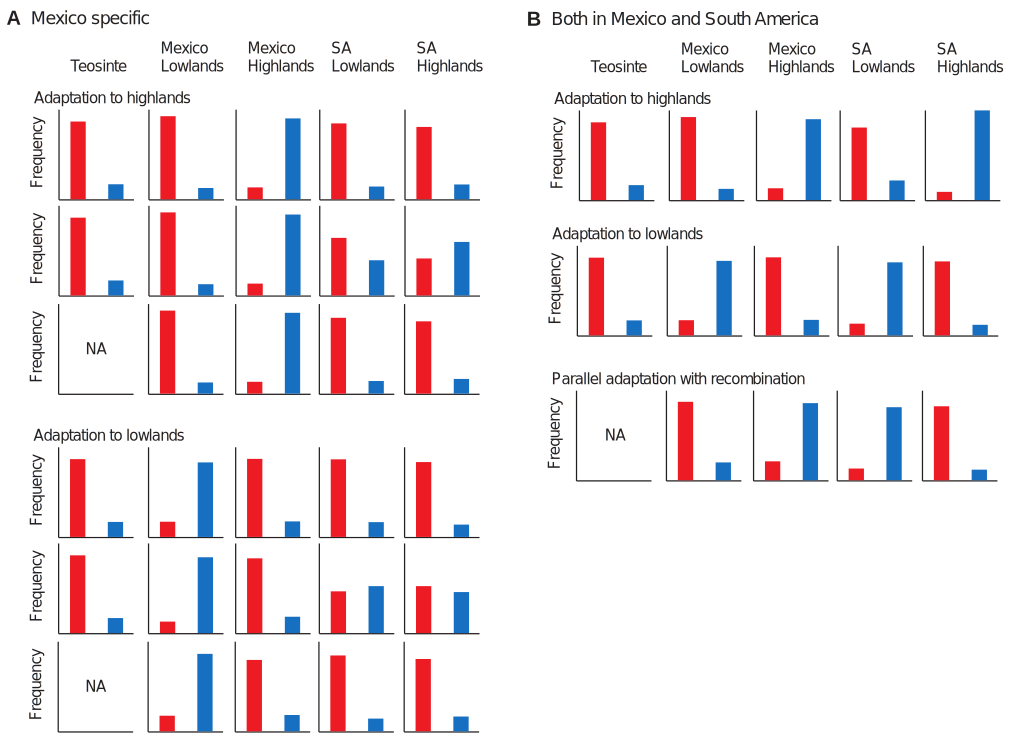
\includegraphics[width=0.49\textwidth]{fig/Fig7}
   \renewcommand{\baselinestretch}{0.9}
   \vspace{-3mm}
   \caption{Illustration for the typical patterns of allele frequency changes in teosinte and maize populations.  Red and blue bars represent the frequencies of putative ancestral and derived alleles, respectively.  (A) The pattern of allele frequencies in the SNPs with Mexico-specific significant $F_{ST}$ \emph{P}-values.  (B) The pattern of allele frequencies in the SNPs with significant $F_{ST}$ \emph{P}-values both in Mexico and South America.}
\vspace{-6mm}
    \label{tes2}
  \end{center}
\end{figure}
%%%%%%%%%%%%%%%%%%%%%%%%%%%%%%%%%%%%%%%%%% FIGURE









%We obtained teosinte (both  and \emph{mexicana}) SNPs in 46 of 56 SNPs from .  39 SNPs exhibited polymorphisms in teosinte, indicating selective sweep from standing genetic variation.  The other seven SNPs showed monomorphic in teosinte.  Only in two of seven SNPs, the frequencies of derived alleles were increased in highland populations. 


%%%%%%%%%%%%%%%%%%%%%%%%%%%%%%%%%%%%%%%%%%%%%%%%%%%%%%%%%%%%
\renewcommand{\arraystretch}{1.1}
\begin{table}[tb]

\begin{center}
 \caption[]{Introgression from \emph{mexicana}\hspace*{0.3cm}}
  \textbf{}\\[-2mm]
{\fontsize{7}{11}\sf
    \begin{tabular}{lcccccccl} 
    \hline
       & & \\[-3mm]
Mexico     & \multicolumn{3}{c}{Number of SNPs}  \\
                                  & Significant & NS & Proportion  \\
Introgressed regions & 149   &   1,918     & 0.072\\ 
Others                        & 872   &  73,578    & 0.011\\
      \hline
    & & \\[-3mm]
South America     & \multicolumn{3}{c}{Number of SNPs} \\
                                  & Significant & NS & Proportion  \\
Introgressed regions & 44   &   1703     & 0.025\\ 
Others      &703   &  60342    & 0.012\\[1mm]
    \hline
  %\multicolumn{4}{l}{$^{a}$ \textcolor{red}{Maybe we should use the number of genetic unit.}}\\
  % \multicolumn{4}{l}{$^{a}$ \textcolor{red}{Sum of the number of SNPs != 91,779 because I excluded SNPs exhibiting}}\\[-0.5mm]
  % \multicolumn{4}{l}{ \textcolor{red}{     monomorphic in Mexico or in South America.}}\\
    \end{tabular}
    \label{mex}  % caption is needed to make this work
}
\end{center}
\end{table}
\renewcommand{\arraystretch}{1}
%%%%%%%%%%%%%%%%%%%%%%%%%%%%%%%%%%%%%%%%%%%%%%%%%%%%%%%%%%%%


%%%%%%%%%%%%%%%%%%%%%%%%%%%%%%%%%%%%%%%%%%%%%%%%%%%%%%%%%%%%
\renewcommand{\arraystretch}{1.1}
\begin{table}[tb]

\begin{center}
 \caption[]{Tanja's $F_{CT}$ between \emph{parviglumis} and \emph{mexicana}\hspace*{0.3cm}}
  \textbf{}\\[-2mm]
{\fontsize{7}{11}\sf
    \begin{tabular}{lcccccccl} 
    \hline
       & & \\[-3mm]
Mexico     & \multicolumn{3}{c}{Number of SNPs}  \\
                                  & Significant & NS & Proportion  \\
Significant $F_{CT}$ & 31   &   331     & 0.086\\ 
NS                        & 373   &  18,419    & 0.020\\
      \hline
    & & \\[-3mm]
South America     & \multicolumn{3}{c}{Number of SNPs} \\
                                  & Significant & NS & Proportion  \\
Significant $F_{CT}$ & 12   &   325     & 0.036\\ 
NS                                & 250   &  17,401    & 0.014\\[1mm]
    \hline
  %\multicolumn{4}{l}{$^{a}$ \textcolor{red}{Maybe we should use the number of genetic unit.}}\\
  % \multicolumn{4}{l}{$^{a}$ \textcolor{red}{Sum of the number of SNPs != 91,779 because I excluded SNPs exhibiting}}\\[-0.5mm]
  % \multicolumn{4}{l}{ \textcolor{red}{     monomorphic in Mexico or in South America.}}\\
    \end{tabular}
    \label{tanja}  % caption is needed to make this work
}
\end{center}
\end{table}
\renewcommand{\arraystretch}{1}
%%%%%%%%%%%%%%%%%%%%%%%%%%%%%%%%%%%%%%%%%%%%%%%%%%%%%%%%%%%%

\subsection*{Comparison to theory}
\plr{need discussion of choices of selection coefficients?}

% # \mutrate computation:
% A <- 500; rho <- 5000; sb <- 10^(-(1:4)); xisq <- 50
% sapply( 10^c(-5,-8), function (mu) mu * (2 * rho * A * sb)/xisq )

Computing the rate $\mutrate$ at which newly adapted alleles arise in the population,
with at total population of $A \rho = 2.5 \times 10^6$ and an offspring variance of $\xi^2 = 50$,
we get that even if there is strong selection for the allele at high elevation ($s_b=0.1$),
then a single-base mutation with mutation rate $\mu=10^{-8}$ would still take at least 10,000 generations to appear and fix.
On the other hand, a kilobase-sized target with mutation rate $\mu=10^{-5}$
with this selection coefficient would fix in only 10 generations,
while more weakly selected alleles with $s_b$ of $10^{-2}$ or $10^{-3}$ would take hundreds or thousands of generations, respectively.
(note: at these values $\Tmut = 1/\mutrate = \mu s_b \times 10^5$.)

% # Tmig computation:
% A <- 500; rho <- 5000; sm <- 10^(-(1:4)); xisq <- 50; sigma <- 2
% 1/(sqrt(2*sm)/sigma)
% sapply( 1000*(1:4), function (R) 1 / ( A * rho * ( sqrt(2*sm) / xisq ) * exp(- sqrt(2*sm)*R/sigma ) ) )
% Ne <- (561/10^5)*A*rho 
% Ne  # = 14025
% sapply( 1000*(1:4), function (R) 1 / ( Ne * exp(- sqrt(2*sm)*R/sigma ) ) )

From the demographic model above
we have estimated that $\sigma \approx 2$ kilometers per generation,
so with $10^{-1} \ge s_m \ge 10^{-4}$ the distance $\sigma/\sqrt{2s_m}$ over which \eqref{eqn:migrate} decays 
is still short: between 4 and 150 kilometers.
\plr{put bounds on $\sigma$}
The area of the Andean highlands is about 500 km$^2$ \plr{is this right???}
which we estimate would be planted from around $N=14,000$ plants each year \plr{add more details here or above}.
Since the Mexican and Andean highlands are around 4,000 km apart,
at $s_m=10^{-3}$ the time needed for this to occur is $\Tmig \approx 5 \times 10^{34}$ generations.
In other words, from these calculations it is almost impossible that an allele that is deleterious at low elevation with $s_m=10^{-3}$ 
would ever transit from the Mexican to the Andean highlands.
If the selection against the allele is even weaker ($s_m=10^{-4}$) it is still expected to take $\Tmig = 1.8 \times 10^8$ generations.
However, shorter distances could be transited by very weakly deleterious alleles --
if $R$ is 1,000 km (or if $\sigma$ is four times larger)
then with $s_m=10^{-4}$ the time $\Tmig$ is about 1.6 generations --
so, adaptation by migration is certain.
However, with even $s_m=10^{-3}$ it is still $2.3 \times 10^6$ generations.

\plr{Here's my conclusions from these calculations.  But, maybe I'm missing something; I want to check more; tell me if anything seems awry.}
It seems unlikely that any alleles that are adaptive in the highlands and deleterious at all in the lowlands
would have transited central America by undirected (diffusive) sharing of seed.
The conclusions could change if we drastically underestimate the rate of very long distance sharing of seed,
e.g.\ if sharing across hundreds of kilometers was common at some point.

Both calculations are very pessimistic about the chance of shared single-base changes through either migration or independent mutation.
However, independent mutations could be expected in kilobase-size targets,
suggesting there might be signal for genes that share adaptive changes.

\plr{mesh this with data analysis\dots}

\section*{Conclusions}
1. We successfully inferred demography and detected the candidates of adaptive loci to highland climates in Mexico and South America by utilizing GBS and 55-k chip.

2. The main conclusion is parallel adaptation is rare in maize highland adaptation.

brabrabra...
%I wanna be the minority$\sim$ \jri{????} \mbh{Green Day fan?}\comst{Yup}

\begin{acknowledgments}
  We appreciate P. Morrell and the members of R-I lab and Coop lab for helpful comments.  
  Funding: USDA.
\end{acknowledgments}


%Note that a SNP with significant \emph{P} value is not necessarily the causative variant because we cannot rule out the possibility that the SNP is just linked to the true causative one.  

%, or the two SNPs are linked to the causative SNPs and recombination .

%    The distance of genetic units would be fairly long, compared to the rapid decay of linkage disequilibrium in maize (roughly 100 bp; Supp Fig. X) \cite[]{Tenaillon_2001_11470895}.  We just assumed that SNPs within a genetic unit have the same functional effect or link to the functional SNP, and based on this assumption, we screened SNPs showing Pattern C of parallel adaptation in Fig.~\ref{fig1}.  \textcolor{red}{Do you have a better idea?}  \jri{i like this but i think we need to be more explicit about relating our analyses back to the patterns.  are we doing this because of linkage or because of biology or both?} \mbh{It might be a good idea to mention linkage to the heuristic set up in Figure 1} 

% \jri{ so this is worth thinking about.  what do we call it if the same SNP was selected but in alternate directions?  i think you need to explain "recombination" further.  i assume you mean that both snp alleles occurred on some background that was then selected in parallel?  since we don't know what SNP was selected how do we categorize this?  Also, somewhere we need to make clear that our different models of parallel adaptation assume that if we see high $F_{ST}$ in two pops that it's because that snp is selected for.  It's just as possible to have the same SNP allele selected in both pops but because it was on different backgrounds! }

% \textcolor{red}{Parallel adaptation in lowland populations also occurred!!} \jri{ not sure how we know this was parallel adaptation in lowland... could be ancestral snp on a derived background (recombination), could be the ancestral allele is suddenly beneficial in a highland habitat (parallel adaptation in highland) or that the new derived allele is beneficial in lowland (parallel adaptation in lowland).  can we distinguish among these (or other) options? }

%Note that the result was not changed when using working gene set. 
%\jri{need to add working gene set not changing result into text.}

%A lot of adaptive SNPs are from standing variation.  That was confirmed by SNPs of teosinte in Hapmap v2. 

%\jri{is standing variation defined in teosinte or should it be defined in lowland ancestral pop? some SNPs that are monomorphic in teo might have been polymorphic in lowland ancestor? } \mbh {It seems if we're talking about highland adaptation from standing variation, it has to be from variation in lowland maize}





%\subsection*{Check overlap with QTL regions} \jri{ skip both these for now}

%\subsection*{Maize cys}
















\bibliography{MZpara1,MZpara2,plr-hilo}
\bibliographystyle{geneticsT2}

\end{document}





%%%%%%%%%%%%%%%%%%%%%%%%%%%%%%%%%%%%%%%%%%%%%%%%%%%%%%%%%%%%
\renewcommand{\arraystretch}{1.1}
\begin{table}[tb]

\begin{center}
 \caption[]{Parallel adaptation\hspace*{0.3cm}}
  \textbf{}\\[-2mm]
{\fontsize{7}{11}\sf
    \begin{tabular}{lllcccccl} \hline
       & & \\[-3mm]
     Description  & Number of genetic units\\[0.1cm]
    \hline
Pattern A or B     & 45 \\
Pattern C from standing variation & 16\\ 
Pattern C from standing variation and & 2\\
\ \ vi new mutations & \\
Total & 63\\[1mm]
    \hline
  \multicolumn{2}{l}{$^{a}$ \textcolor{red}{In this table, I did not use the information of teosinte polymorphisms.}}\\
    \end{tabular}
    \label{paraGU}  % caption is needed to make this work
}
\end{center}
\end{table}
\renewcommand{\arraystretch}{1}
%%%%%%%%%%%%%%%%%%%%%%%%%%%%%%%%%%%%%%%%%%%%%%%%%%%%%%%%%%%%


% pre
%%%%%%%%%%%%%%%%%%%%%%%%%%%%%%%%%%%%%%%%%%%%%%%%%%%%%%%%%%%%
\renewcommand{\arraystretch}{1.1}
\begin{table}[tb]

\begin{center}
 \caption[]{Parallel adaptation\hspace*{0.3cm}}
  \textbf{}\\[-2mm]
{\fontsize{7}{11}\sf
    \begin{tabular}{lllcccccl} \hline
       & & \\[-3mm]
     Description  & Number of genetic units\\[0.1cm]
    \hline
Parallel adaptation     &  \\
Pattern A or B     & 45 \\
Pattern C from standing variation & 16\\ 
Pattern C from standing variation and & 2\\
\ \ vi new mutations & \\
Total & 63\\
      \hline
    & & \\[-3mm]
Only Mexico     &  \\
From standing variation & 635 \\
New mutations & 65 \\
Both mechanisms & 16 \\
Total & 716\\
      \hline
    & & \\[-3mm]
Only South America     &  \\
From standing variation & 458 \\
New mutations & 36 \\
Both mechanisms & 4 \\
Total & 498\\[1mm]
    \hline
  \multicolumn{2}{l}{$^{a}$ \textcolor{red}{Check teosinte polymorphisms on Hapmap2 later.}}\\
    \end{tabular}
    \label{paraGU}  % caption is needed to make this work
}
\end{center}
\end{table}
\renewcommand{\arraystretch}{1}
%%%%%%%%%%%%%%%%%%%%%%%%%%%%%%%%%%%%%%%%%%%%%%%%%%%%%%%%%%%%

